\scanpage{84}

% top, lines 1–2
exactement -- ceci correspond à $4$ carrés de $\overline{=}$ centre $a$).

% upper, question
\uline{Question} Quels sont les graphes finis qui ont \unsure{aussi|ainsi} une ``enveloppe'' \inserted{pseudo} \unsure{trialitaire|trilatère} ? Exemples.

% upper left, rounded outline beside examples
\figure{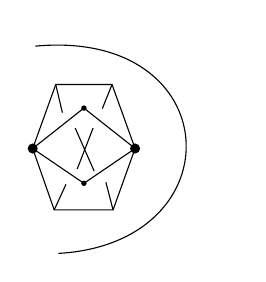
\begin{tikzpicture}[scale=.65]
\draw (-.55,1.25)--(.55,1.25)--(1,0)--(.57,-1.2)--(-.58,-1.2)--(-1,0)--cycle;
\draw (-1,0)--(0,.79)--(1,0)--(0,-.68)--cycle (-.55,1.25)--(-.42,.7) (.55,1.25)--(.36,.78) (-.58,-1.2)--(-.35,-.7) (.57,-1.2)--(.43,-.66);
\draw (-.17,.4)--(.2,-.44) (.18,.4)--(-.13,-.4);\fill (-1,0) circle (2.8pt) (1,0) circle (2.8pt) (0,.79) circle (1.5pt) (0,-.68) circle (1.5pt);
\draw (-.95,2) .. controls (2.8,2.35) and (3,-1.85) .. (-.5,-2.05);
\end{tikzpicture}}

% upper middle, six examples
\diagram{\begin{tikzcd}[ampersand replacement=\&,row sep=1.2em,column sep=.9em,cells={font=\scriptsize}]
\bullet\arrow[d]\&\rule{1.3em}{1.5pt}\arrow[d]\&
\tikz[baseline=-.6ex]{\draw (0,0) rectangle (.5,.48);\draw[very thick] (0,0)--(.5,0);}\arrow[d]\&
\tikz[baseline=-.6ex]{\draw (90:.3)--(18:.3)--(-54:.3)--(-126:.3)--(162:.3)--cycle;\draw[very thick] (-54:.3)--(-126:.3);}\arrow[d]\&
\tikz[baseline=-.6ex]{\draw (100:.3)--(30:.3)--(-38:.3)--(-114:.3)--(168:.3)--cycle;\draw[very thick] (100:.3)--(30:.3)--(-38:.3)--(-114:.3);}\arrow[d]\&
\tikz[baseline=-.6ex]{\draw[very thick] (-.2,.3)--(.2,.3) (-.2,-.2)--(.2,-.2);\draw[thin,rounded corners=3pt] (-.34,-.25)--(-.42,.12)--(-.25,.48)--(.32,.47)--(.42,.16)--(.29,-.27)--(.14,-.38)--cycle;}\arrow[d]\\
\bullet\&\unsure{\text{arête}}\&\text{pavé}\&\text{pavé}\&\unsure{\text{carré}}\&
\tikz[baseline=-.6ex]{\draw (-.14,0)--(.17,.46)--(-.03,.46)--(.12,0)--cycle;}
\end{tikzcd}}

% upper right and below examples
(et bien sûr les complexes \inserted{pseudo} trialitaires eux-$\overline{=}$s) et les \deleted{de graphes} graphes intermédiaires entre ceux-ci et leur enveloppe

% above middle examples
Regarder p.ex. \unsure{les}

% middle, upper row of examples
\figure{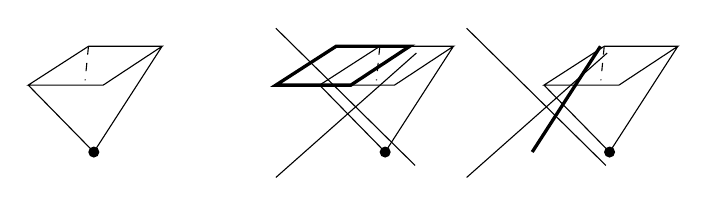
\begin{tikzpicture}[x=.85cm,y=.85cm]
\foreach \k in {0,3.7,6.55}{\begin{scope}[xshift=\k cm]
\draw (0,0)--(.9,.58)--(2,.58)--(1.12,0)--cycle (0,0)--(.98,-1)--(2,.58);\draw[dashed] (.9,.58)--(.85,.07);\fill (.98,-1) circle (2pt);\end{scope}}
\draw[very thick] (3.7,0)--(4.6,.58)--(5.7,.58)--(4.82,0)--cycle (7.53,-1)--(8.55,.58);
\foreach \k in {3.7,6.55}{\draw (\k,.85)--({\k+2.08},-1.2) (\k,-1.38)--({\k+2.1},.48);}
\end{tikzpicture}}

% middle left, below Regarder
\deleted{\unsure{graphes}} \deleted{Regarder}

% middle, lower row of examples
\figure{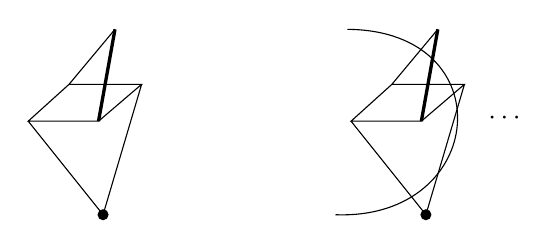
\begin{tikzpicture}[x=.72cm,y=.72cm]
\foreach \k in {0,4.1}{\begin{scope}[xshift=\k cm]\draw (0,0)--(.72,.65)--(2,.65)--(1.24,0)--cycle (0,0)--(1.32,-1.65)--(2,.65) (.72,.65)--(1.53,1.62);\draw[very thick] (1.53,1.62)--(1.24,0);\fill (1.32,-1.65) circle (2pt);\end{scope}}
\draw (5.63,1.62) .. controls (8.4,1.6) and (8.1,-1.75) .. (5.42,-1.65);
\node at (8.4,.05) {$\cdots$};
\end{tikzpicture}}

% across middle
\noindent\rule{\linewidth}{.35pt}

% lower right, three shape labels
\figure{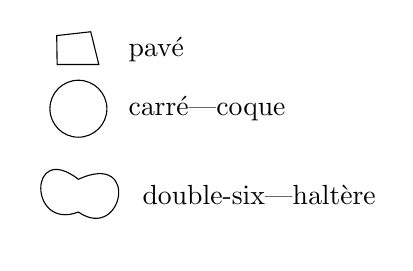
\begin{tikzpicture}[scale=.54]
\draw (-.5,0)--(.48,0)--(.29,.77)--(-.51,.68)--cycle;\node[right] at (.95,.36) {pavé};
\draw (0,-1.04) circle (.67);\node[right] at (.95,-1.04) {\unsure{carré|coque}};
\draw (0,-2.7) .. controls (-1.18,-1.78) and (-1.18,-3.92) .. (0,-3.47) .. controls (1.04,-4.19) and (1.47,-2.02) .. (0,-2.7);\node[right] at (1.28,-3.07) {\unsure{double-six|haltère}};
\end{tikzpicture}}

% lower field, covering diagram and adjacent point clusters
\diagram{\begin{tikzcd}[ampersand replacement=\&,column sep=2em,row sep=2.2em,cells={font=\scriptsize}]
{\times\ \bullet\ \cdot}\& {\substack{\mathrm{Car}_s\simeq\mathrm{hex}_s\\\unsure{\updownarrow|\wr}\\\mathrm{tria}\,\text{ép}}}\arrow[r]\arrow[dl,dash]\&{\substack{\mathrm{Car}_{\mathrm{rep}}\\\unsure{\updownarrow|\wr}\\\mathrm{hex}\,\text{ép}}}\arrow[dl,dash]\arrow[d,bend left=18]\arrow[dll]\\
{\substack{\mathrm{Car}_d\sim\mathrm{hex}_d\\\unsure{\updownarrow|\wr}\simeq\deleted{\unsure{\mathrm{Hex}}}_d\\\mathrm{tria}\,\mathrm{pt}}}\arrow[d,dash]\&
{\substack{\mathrm{Car}_{r'}\simeq\mathrm{hex}_{s*}}}\arrow[l]\arrow[d]\&
{\unsure{\mathrm{Car}_{s*}}}\arrow[dl,dash]\\
{\substack{\mathrm{Car}\\\simeq\mathrm{pav}\,\mathrm{pt}}}\arrow[r,dash]\&\mathrm{Car}_{d*}\&
\end{tikzcd}}

% lower field, miniature figures surrounding diagram
\figure{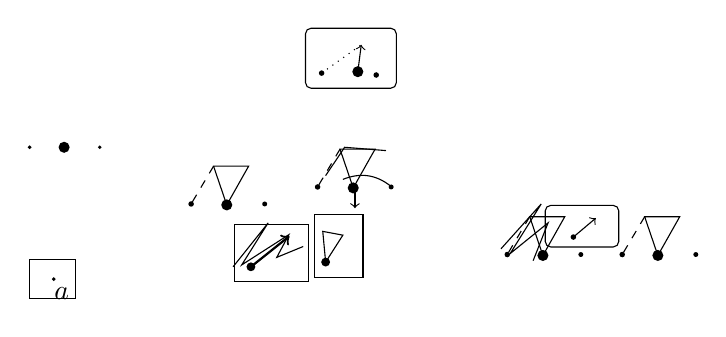
\begin{tikzpicture}[x=.73cm,y=.6cm]
\foreach \x/\r in {0/.7, .6/2,1.22/.7}{\fill (\x,2) circle (\r pt);}
\draw[rounded corners=2pt] (4.8,3.25) rectangle (6.38,4.52);\fill (5.08,3.57) circle (1pt) (5.71,3.6) circle (2pt) (6.03,3.53) circle (1pt);\draw[->] (5.71,3.6)--(5.77,4.17);\draw[dotted] (5.08,3.57)--(5.77,4.17);
\foreach \x/\y in {3.2/1.6,5.4/1.96,8.7/.53,10.7/.53}{\begin{scope}[shift={(\x,\y)}]\draw (0,0)--(.23,-.82)--(.61,0)--cycle;\draw[dashed] (0,0)--(-.39,-.8);\fill (.23,-.82) circle (2pt) (-.39,-.8) circle (1pt) (.89,-.8) circle (.9pt);\end{scope}}
\draw[->] (5.66,1.13)--(5.66,.71);\draw (5.15,1.4)--(5.48,2)--(6.2,1.93);\draw (5.45,1.32) to[bend left] (6.28,1.18);
\draw[rounded corners=2pt] (8.97,-.11) rectangle (10.25,.77);\draw[->] (9.46,.1)--(9.85,.5);\fill (9.46,.1) circle (1pt);
\draw[thin] (8.2,-.15)--(8.9,.8)--(8.36,-.25)--(9.02,.4)--(8.76,-.4);
\draw (0,-1.2) rectangle (.8,-.38);\fill (.42,-.79) circle (.7pt);\node at (.56,-1.1){$a$};
\draw (3.56,-.84) rectangle (4.85,.36) (4.95,-.76) rectangle (5.8,.57);
\fill (3.85,-.53) circle (1.6pt) (5.15,-.43) circle (1.6pt);\draw[->,thick] (3.85,-.53)--(4.52,.12);\draw (5.15,-.43)--(5.45,.14)--(5.1,.22)--cycle;
\draw[thin] (3.54,-.53)--(4.15,.4)--(3.69,-.49)--(4.51,.15)--(4.3,-.33)--(4.76,-.1);
\end{tikzpicture}}

% foot right, four labels
\diagram{\begin{tikzcd}[ampersand replacement=\&,row sep=small]
{\text{\uuline{$\mathrm{Car}$}}_d}\arrow[r,dash]\arrow[d,phantom,"\unsure{\wr\!\vert|\wr}"]\&{\text{\uuline{$\mathrm{Car}$}}}\arrow[dr]\\
\mathrm{hex}_d\arrow[r,dash]\&\mathrm{hex}\&{}
\end{tikzcd}}

% archive sheet number: 83
